\documentclass[12pt, a4paper]{report}
\usepackage[utf8]{inputenc}
\usepackage[T1]{fontenc}
\usepackage[french]{babel}
\usepackage{graphicx}
\usepackage{float}
\usepackage{eurosym}
\usepackage{enumitem}
\usepackage{amsmath}
\usepackage{lipsum}
\usepackage{fancyhdr}
\usepackage{xcolor}
\usepackage{minitoc}
\usepackage{listings}

% Configuration spéciale pour Arduino
\lstset{
	language=C++,
	basicstyle=\ttfamily\footnotesize,
	keywordstyle=\color{blue}\bfseries,
	commentstyle=\color{green!60!black},
	stringstyle=\color{red},
	% Ajout des mots-clés spécifiques à Arduino
	morekeywords={setup, loop, pinMode, digitalWrite, digitalRead, analogRead, analogWrite, Serial, begin, print, println, delay, HIGH, LOW, INPUT, OUTPUT},
	numbers=left,
	numberstyle=\tiny\color{gray},
	stepnumber=1,
	breaklines=true,
	frame=single,
	showstringspaces=false,
	tabsize=4
}

%Entéte
\pagestyle{fancy}
\fancyhf{}
\lhead{
\includegraphics[width=2cm]{Image/logo_Polytech_HORIZ_dijon}}
\rhead{\today}
\cfoot{Page \thepage}
\begin{document}
	\begin{titlepage}
		\centering 
		
\includegraphics[width=0.3\textwidth]{Image/logo_Polytech_HORIZ_dijon}\par\vspace{1cm}
		
		%     En-tête 
		{\scshape\LARGE Polytech Dijon \par}
		\vspace{1cm}
		
		%     Titre 
		\textcolor{blue}{\rule{\linewidth}{0.5mm}} \\[0.4cm] % Ligne horizontale supérieure
		{ \huge \bfseries Mécatronique \\[0.4cm] }
		{\scshape\LARGE Travaux Pratique \par}
		\textcolor{blue}{\rule{\linewidth}{0.5mm}} \\[1,5cm] % Ligne horizontale inférieure
		%     Sous-titre ou nature du document 
		{\Large Compte rendu \par}
		\vspace{2cm}
		%     Auteurs et Superviseurs    
		\begin{minipage}{0.40\textwidth}
			\begin{flushleft} \large
				\emph{Réalisé par :}\\
				ADIDO Caurel\\
				BAKAI Mamalineso\\
				CLOIX Mattys 
			\end{flushleft}
		\end{minipage}
		\hfill
		\begin{minipage}{0.55\textwidth}
			\begin{flushright} \large
				\emph{Supervisé par :} \\
				ABADI Amine \\ 
				
			\end{flushright}
		\end{minipage}
		\vfill 
		% --- Date ---
		{\large \today \par}
	\end{titlepage}
	\newpage
	\tableofcontents
	\newpage
	
	%Inclusion des différents TP
	\chapter{TP1:Présentation et programmation de la carte Arduino}
\minitoc
\newpage
\section{Matériel}

Le projet Arduino a été conçu par une équipe de six développeurs pour offrir une plateforme de création de systèmes électroniques accessible à tous, des débutants aux professionnels.

\begin{figure}[H]
	\centering
	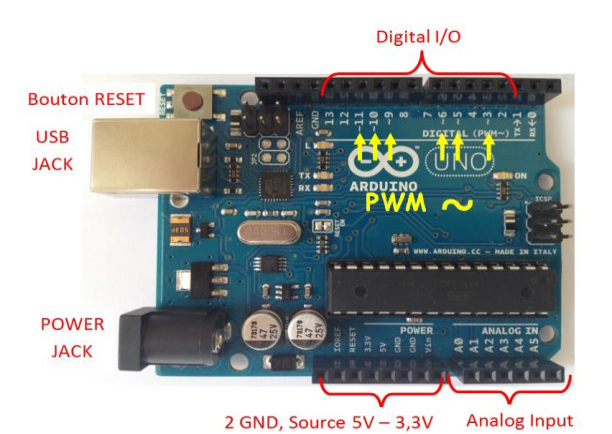
\includegraphics[width=0.7\linewidth]{Image/1.Arduino_Uno}
	\caption{Arduino Uno}
	\label{fig:arduinouno}
\end{figure}

La carte Arduino UNO est un circuit imprimé architecturé autour du microcontrôleur ATmega328. Elle est équipée d'une interface USB permettant une communication directe avec un ordinateur. 

\paragraph{Caractéristiques techniques principales :}
\begin{itemize}
	\item \textbf{Tensions :} Fonctionnement sous 5V, avec une tension d'alimentation recommandée de 7 à 12V.
	\item \textbf{Performances :} Horloge cadencée à 16~MHz et mémoire Flash de 32~Ko.
	\item \textbf{Courant :} Jusqu'à 40~mA par broche d'entrée/sortie (50~mA pour la broche 3.3V).
	\item \textbf{Brochage :}
	\begin{itemize}
		\item \emph{Entrées analogiques :} A0 à A5
		\item \emph{Entrées/Sorties numériques :} 2 à 19
		\item \emph{Sorties PWM (analogiques simulées) :} 3, 5, 6, 9, 10, 11
	\end{itemize}
\end{itemize}
\section{Le logiciel Arduino}
La programmation de la carte Arduino nécessite un logiciel pour écrire le code puis le transférer. Nous utiliserons pour cela Arduino IDE, une solution gratuite et open source.
\begin{figure}[H]
	\centering
	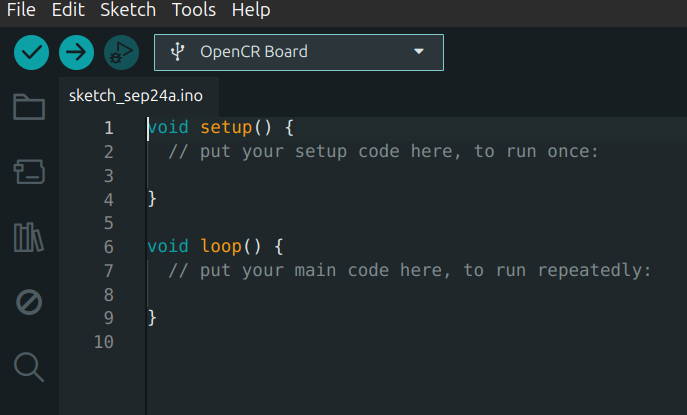
\includegraphics[width=0.7\linewidth]{Image/1.Interface_IDE}
	\caption{Interface Arduino IDE}
	\label{fig:interfaceide}
\end{figure}

\section{Manipulation}
\subsection{Manipulation 1 : Une LED qui clignote}
Le but de cette première manipulation est de nous familiariser avec la carte Arduino Uno en faisant simplement clignoter une LED.
\begin{figure}[H]
	\centering
	\begin{minipage}{0.48\textwidth}
		\centering
		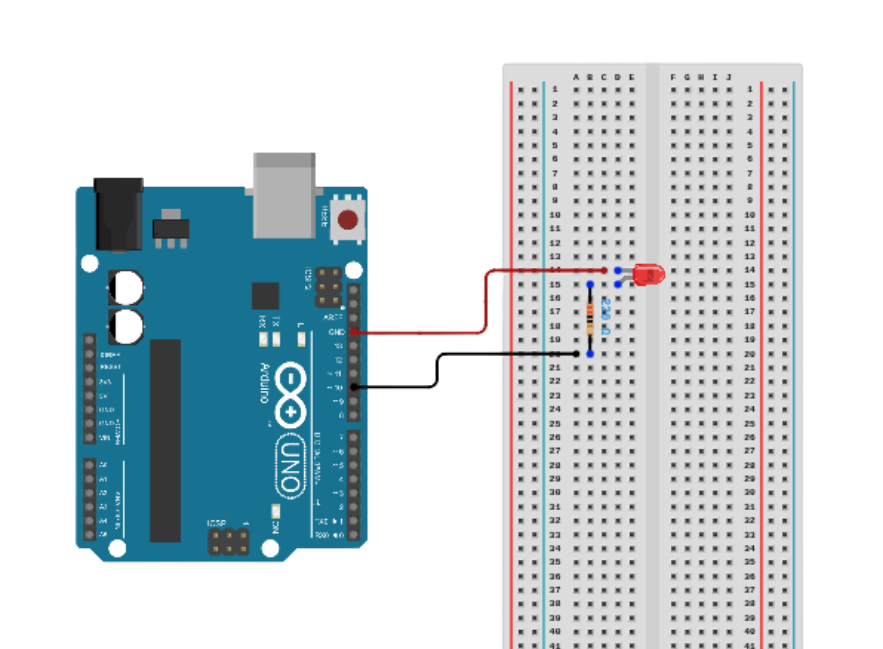
\includegraphics[width=\linewidth]{Image/1.Schéma_Manip1}
		\caption{Schéma Manipulation 1}
		\label{fig:schemamanip1}
	\end{minipage}\hfill
	\begin{minipage}{0.48\textwidth}
		\centering
		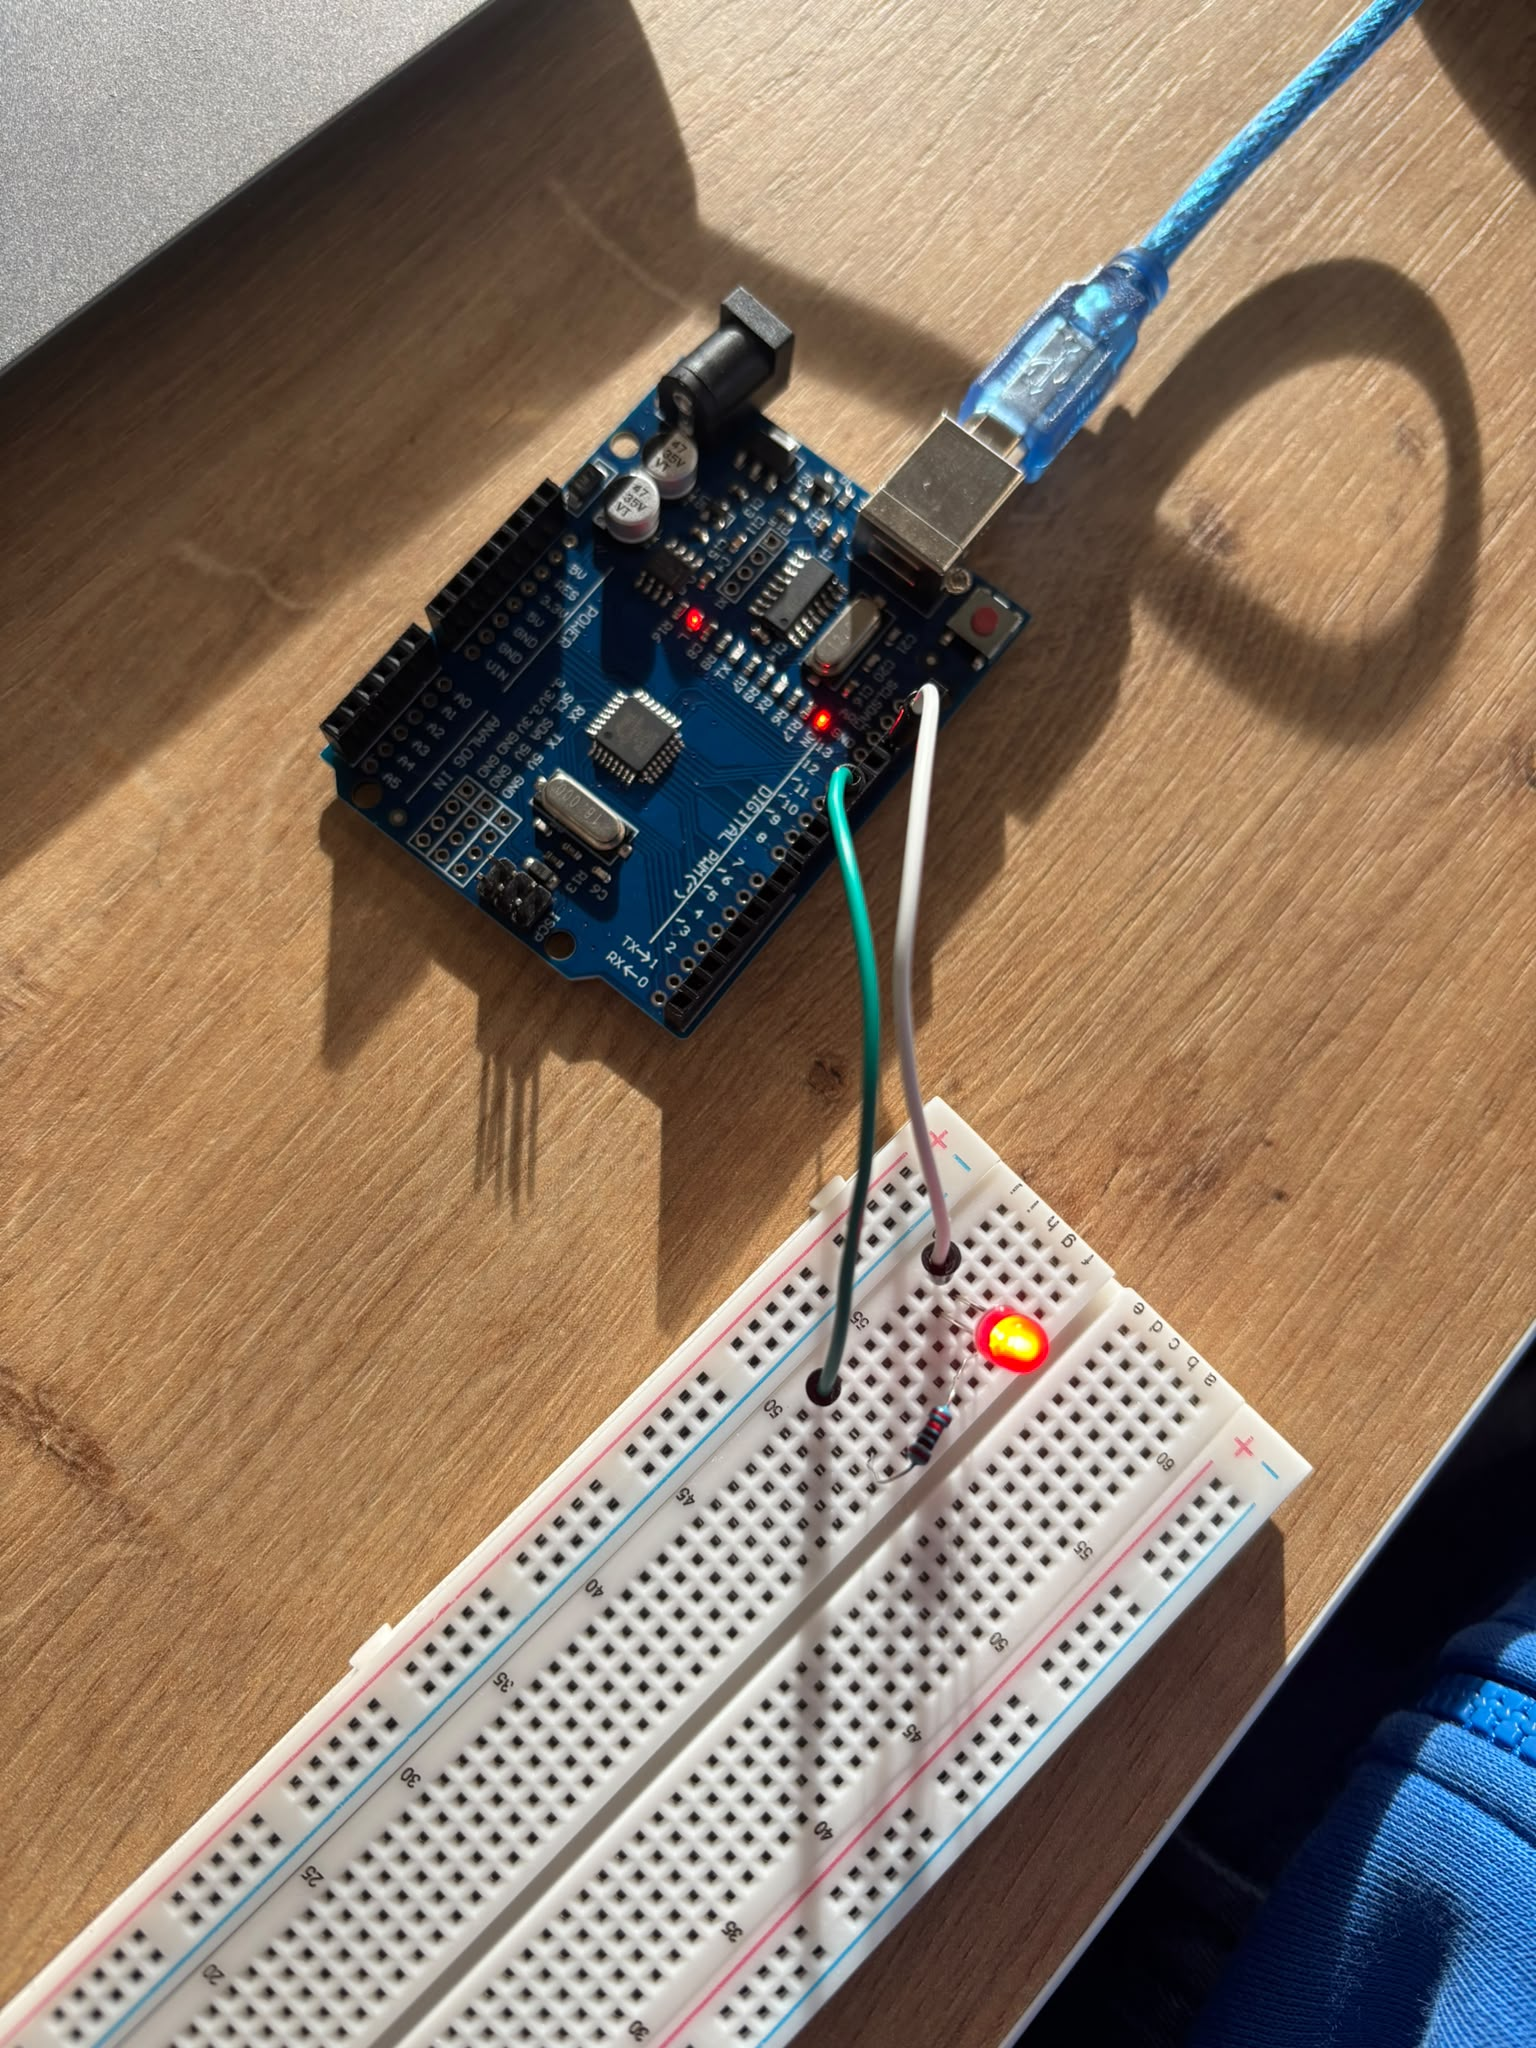
\includegraphics[width=\linewidth]{Image/1.Photo_manip1}
		\caption{Photo Manipulation 1}
		\label{fig:photomanip1}
	\end{minipage}
\end{figure}
Voici le code qui nous est donné pour tester notre LED
\begin{lstlisting}
	void setup() {		
		pinMode(10, OUTPUT); // ici nous definissons notre pin 10 comme une sortie 		
	}	
	void loop() {		
		digitalWrite(10, HIGH); // ici on allume la LED
		delay(500); // on attends 500 millisecondes
		digitalWrite(10, LOW);
		delay(500); // on attends 500 millisecondes		
	}
		
\end{lstlisting}
\textbf{Observation :} Nous remarquons bien que la LED clignote. 

\subsection{Manipulation 2 : Trois LED qui clignote}
Dans cette partie du TP, nous devons apprendre à gérer trois LED en même temps avec notre Arduino.
\begin{figure}[H]
	\centering
	% Première image à gauche (48% de la largeur de la page)
	\begin{minipage}{0.48\textwidth}
		\centering
		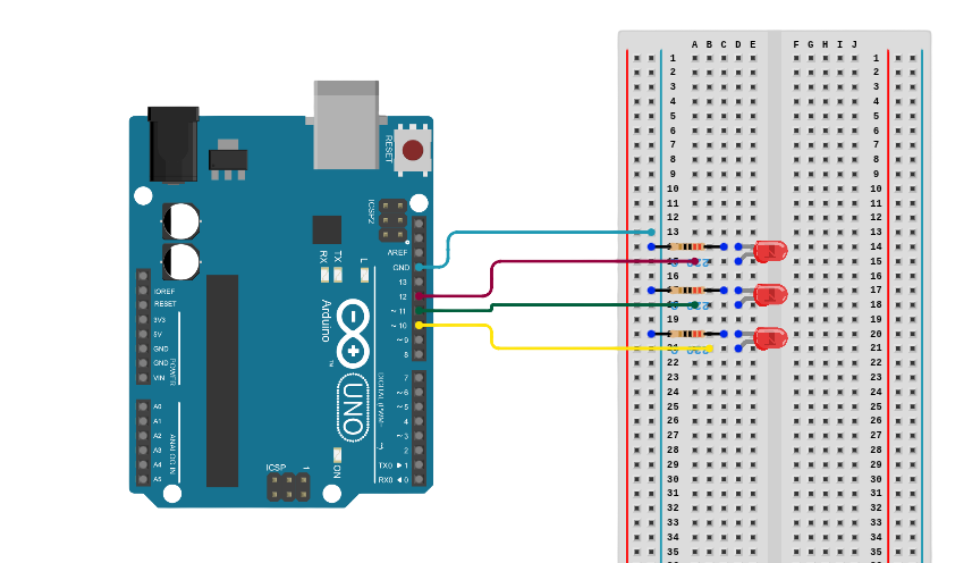
\includegraphics[width=\linewidth]{Image/1.Schéma_manip2}
		\caption{Schéma manipulation 2}
		\label{fig:schemamanip2}
	\end{minipage}\hfill
	% Seconde image à droite (48% de la largeur de la page)
	\begin{minipage}{0.48\textwidth}
		\centering
		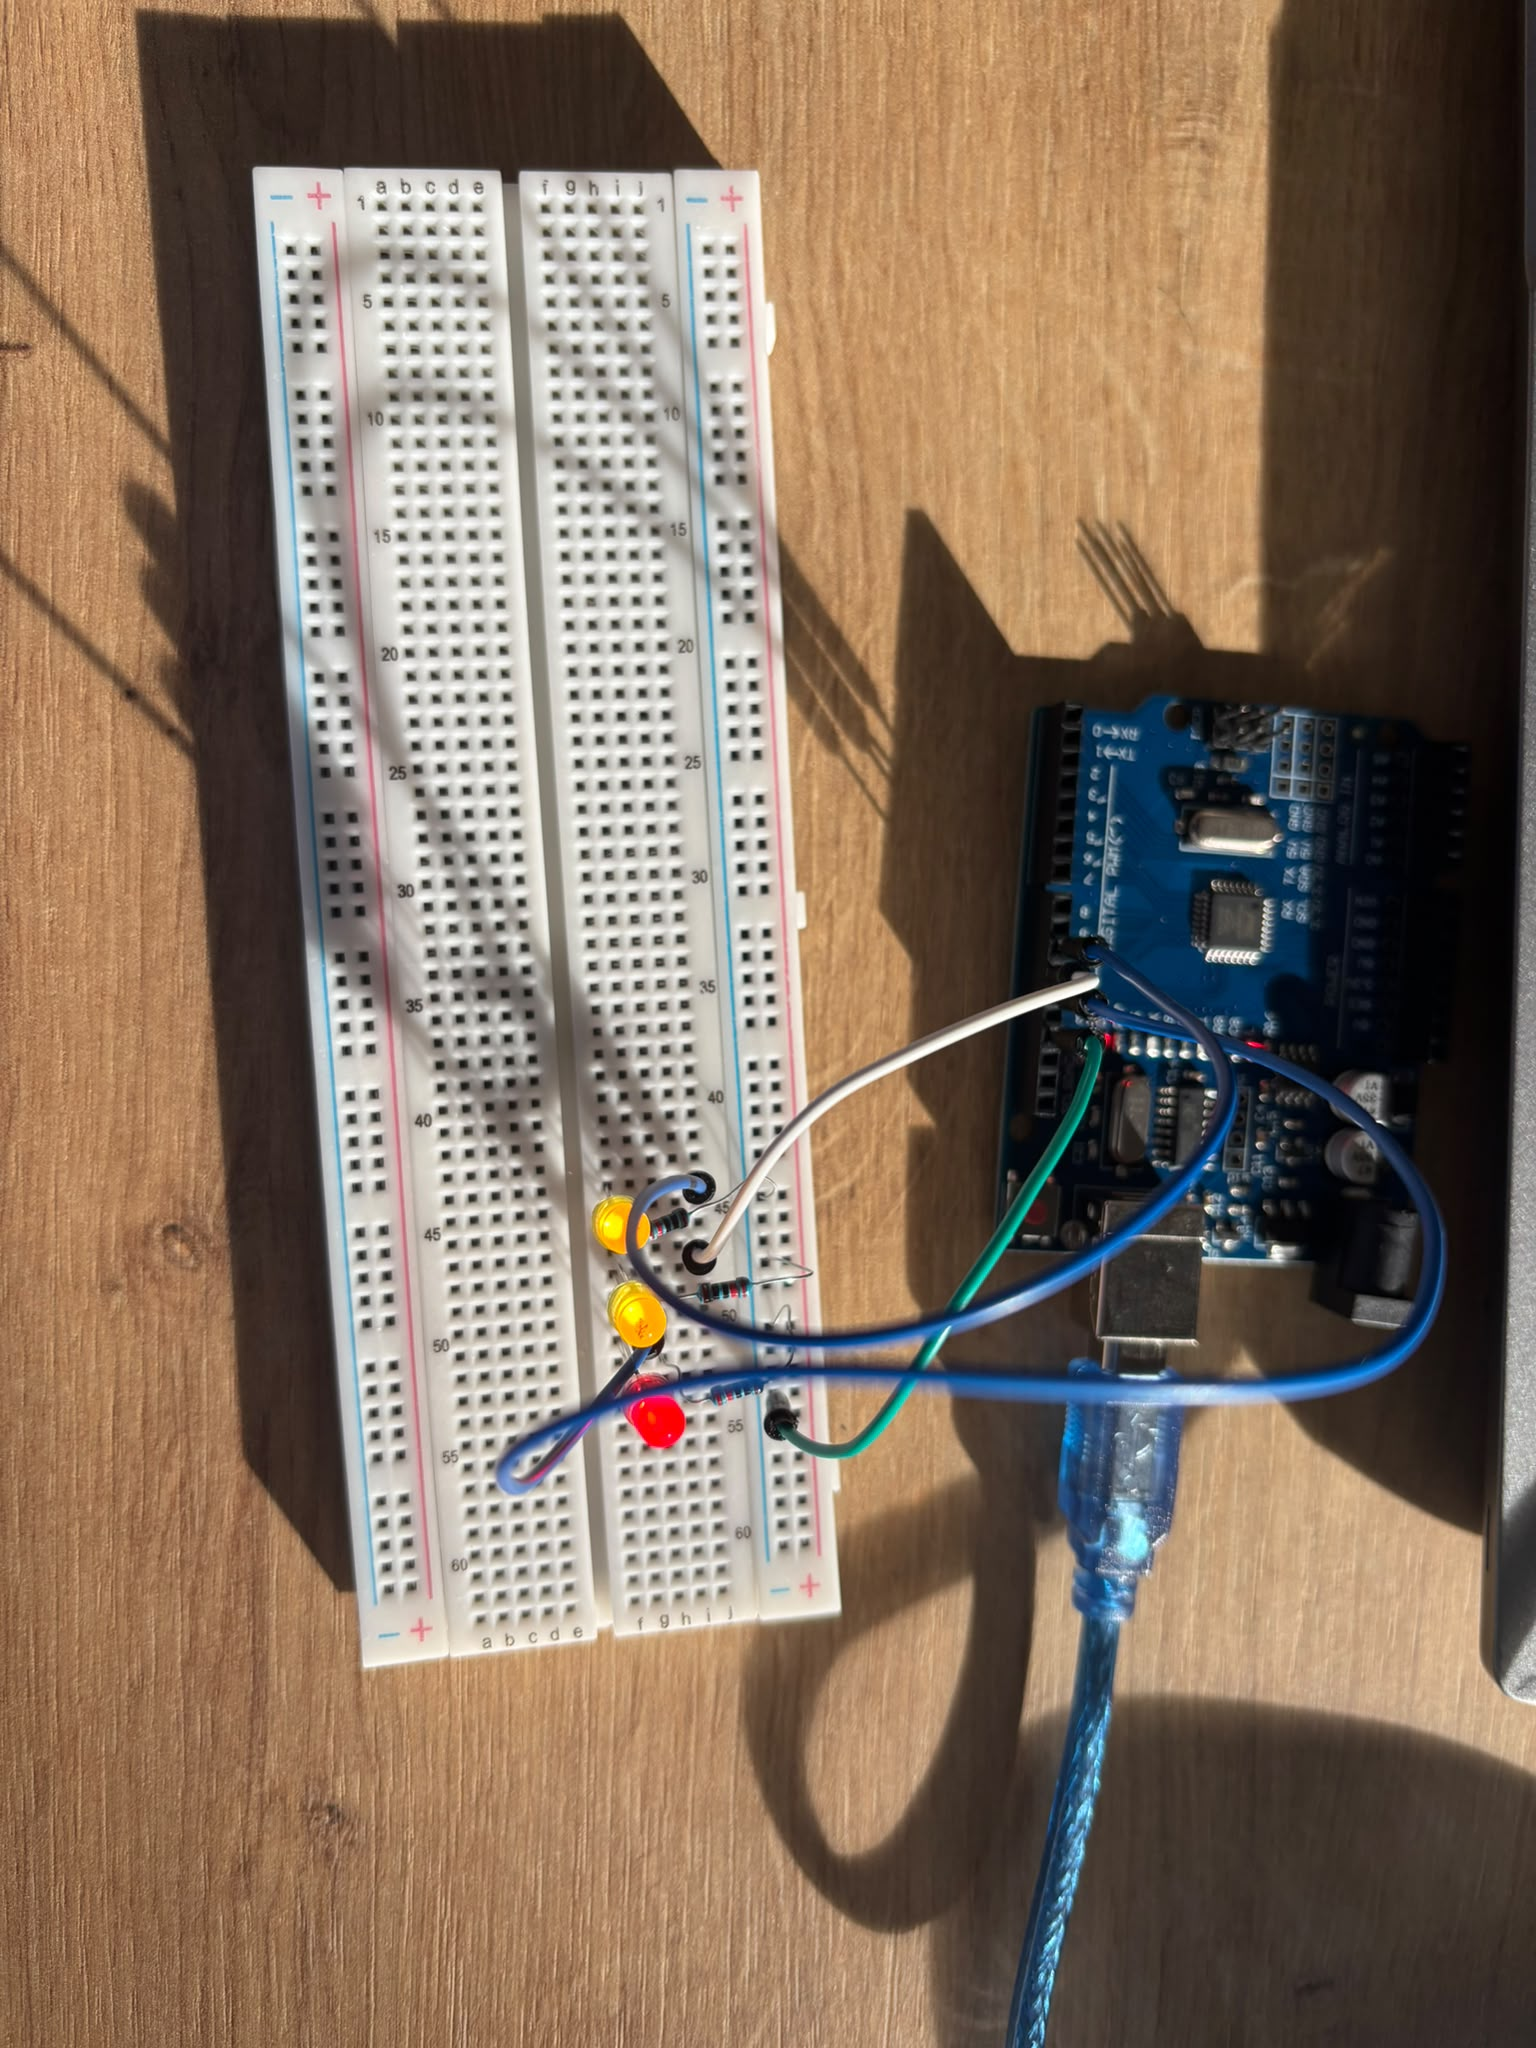
\includegraphics[width=\linewidth]{Image/1.Photo_manip2}
		\caption{Photo Manipulation 2}
		\label{fig:photomanip2}
	\end{minipage}
\end{figure}
Voici notre code pour faire code pour faire clignoter les trois LED
\begin{lstlisting}	
	void setup() {
		pinMode(10, OUTPUT); // ici nous definissons notre pin 10 comme une sortie 
		pinMode(11, OUTPUT); // ici nous definissons notre pin 11 comme une sortie 
		pinMode(12, OUTPUT); // ici nous definissons notre pin 12 comme une sortie 
	}
	void loop() {
		digitalWrite(10, HIGH); // ici on allume la LED
		digitalWrite(11, HIGH); // ici on allume la LED
		digitalWrite(12, HIGH); // ici on allume la LED
		
		delay(500); // on attends 500 millisecondes
		
		digitalWrite(10, LOW);
		digitalWrite(11, LOW);
		digitalWrite(12, LOW);
		
		delay(500); // on attends 500 millisecondes		
	}	
\end{lstlisting}
\textbf{Observation :} Nous remarquons que les trois LED s'allume simultanément.\\
Ensuite nous devons faire en sorte que les trois Led s'allume avec alternance. Voici le code pour faire cela. 
\begin{lstlisting}	
	void loop() {		
		digitalWrite(10, HIGH); // ici on allume la LED
		delay(500); // on attends 500 millisecondes
		digitalWrite(10, LOW); // ici on allume la LED
		
		delay(500);
		
		digitalWrite(11, HIGH); // ici on allume la LED
		delay(500); // on attends 500 millisecondes
		digitalWrite(11, LOW); // ici on allume la LED
		
		delay(500);
		
		digitalWrite(12, HIGH); // ici on allume la LED
		delay(500); // on attends 500 millisecondes
		digitalWrite(12, LOW); // ici on allume la LED
		
		delay(500);
	}	
\end{lstlisting}
\textbf{Observations :} Nous remarquons bien une alternance dans l'allumage des LED.\\
Pour la prochaine questions nous devons réaliser un feu tricolore avec nos trois LED de couleur. Voici alors notre code pour réaliser cela.
\begin{lstlisting}		
	#define LED_rouge  12 // ici nous renommons nous leds pour mieux les distinguer
	#define LED_vert   11
	#define LED_orange 10	
	void setup() {		
		pinMode(LED_rouge, OUTPUT); 
		pinMode(LED_vert, OUTPUT); 
		pinMode(LED_orange, OUTPUT); 
	}	
	void loop() {
		
		digitalWrite(LED_orange, HIGH); 
		digitalWrite(LED_vert, LOW);
		digitalWrite(LED_rouge, LOW);
		
		delay(1000);
		
		digitalWrite(LED_orange, LOW);
		digitalWrite(LED_vert, LOW);
		digitalWrite(LED_rouge, HIGH);
		
		delay(4000);
		
		digitalWrite(LED_orange, LOW); 
		digitalWrite(LED_vert, HIGH);
		digitalWrite(LED_rouge, LOW);
		
		delay(4000);		
	}		
\end{lstlisting}
\textbf{Observations :} Nous remarquons bien le fait que les LED s'allume a l'image d'un feux tricolore.\\
L'exercice suivant consiste à répéter 15 fois le clignotement d'une seule LED. Pour éviter d'alourdir le programme, nous allons conserver notre structure actuelle et introduire une boucle for. 
\begin{lstlisting}			
	void setup() {
		Serial.begin(9600);
		
		pinMode(10, OUTPUT); 
				
		for(int i=0 ; i <15 ; i++){ // cette boucle for nous permet d'executer le code 15 fois 
			Serial.println(i);
			digitalWrite(10,HIGH);
			delay(500);
			digitalWrite(10,LOW);
			delay(500);			
		}
	}	
	void loop() {		
		// ici on ne mets rien car on souhaite que le code sexecute que 15 fois		
	}
\end{lstlisting}
\textbf{Observations :} Nous vérifions bien que la LED s’allume et s’éteint 15 fois.\\
Nous avons désormais un code a tester.
\begin{lstlisting}				
	int ledPin = 10; //On renomme la broche 10 en "ledPin"
	int timer = 100; //On definit une duree de 0,1 seconde pour la variable timer
	
	void setup() { pinMode(ledPin, OUTPUT); }
	
	void loop() {		
		// LED a 0%.
		analogWrite(ledPin, 0);
		delay(timer);
		// LED a 19.6%.
		analogWrite(ledPin, 50);
		delay(timer);
		// LED a 39.2%.
		analogWrite(ledPin, 100);
		delay(timer);
		// LED a 58.8%.
		analogWrite(ledPin, 150);
		delay(timer);
		// LED a 78.4%.
		analogWrite(ledPin, 200);
		delay(timer);
		// LED a 100%.
		analogWrite(ledPin, 255);
		delay(timer); }
\end{lstlisting}
\textbf{Observations :} La LED augmente en luminosité jusqu’à s'éteindre.\\
Maintenant que nous avons compris ce précedent code nous devons jouer avec la luminosité des Trois différente LED.
\begin{lstlisting}					
	int ledPin = 10; //On renomme la broche 10 en "ledPin"
	int timer = 100; //On definit une duree de 0,1 seconde pour la variable timer
	
	void setup() {
		pinMode(ledPin, OUTPUT);
	}
	
	void loop() {
		analogWrite(10, (255*10)/100); // ici on definit la luminosite de la led_10 a 10% de 255
		analogWrite(11, (255*40)/100); // ici on definit la luminosite de la led_11 a 40% de 255
		analogWrite(12, (255*80)/100); // ici on definit la luminosite de la led_12 a 80% de 255
		
		delay(timer);
		
		analogWrite(10, (255*0)/100); // ici on definit la luminosite de la led_10 a 0% de 255
		analogWrite(11, (255*0)/100); // ici on definit la luminosite de la led_11 a 0% de 255
		analogWrite(12, (255*0)/100); // ici on definit la luminosite de la led_12 a 0% de 255		
		
		delay(timer);		
	}
\end{lstlisting}
\textbf{Observations :}Les trois LED clignote mais avec une intensité lumineuse différente.\\
Pour finir avec ce TP nous allons réaliser un chenillard avec nos trois LED. 
\begin{lstlisting}						
	int timer = 500; //On definit une duree de 0,5 seconde pour la variable timer	
	void setup() {
		pinMode(10, OUTPUT);
		pinMode(11, OUTPUT);
		pinMode(12, OUTPUT);
	}	
	void loop() {		
		for (int i = 10 ; i < 13 ; i++) {			
			digitalWrite(i, HIGH);
			delay(timer);
			digitalWrite(i, LOW);			
		}		
	}
\end{lstlisting} 
\textbf{Observations :} Nous observons bien l'allumage des LED de façons successive.
	\chapter{TP2:Utilisation du CAN de l’Arduino}
\minitoc
\newpage
\section{Convertisseur Analogique numérique}
La carte Arduino Uno intègre un unique convertisseur analogique/numérique (CAN) de 10 bits, partagé entre ses 6 entrées (A0 à A5). Il convertit le signal en environ 100 µs pour délivrer une valeur numérique allant de 0 à 1023.
\section{Mesurer une température avec un capteur LM35 et une carte Arduino}
Le LM35 est un capteur de température électronique analogique de précision. Il se présente sous la forme d'un composant à trois broches :
\begin{itemize}
	\item \textbf{VCC} : Alimentation (reliée au 5V)
	\item \textbf{Analog Voltage Out} : Sortie de la tension (reliée à une entrée analogique)
	\item \textbf{GND} : Masse
\end{itemize}
\paragraph{Principe de mesure :}
D'après la fiche technique du composant, la tension de sortie est proportionnelle à la température avec une sensibilité de $10\,\mathrm{mV} / ^{\circ}\mathrm{C}$. Autrement dit, une tension de $1\,\mathrm{V}$ correspond à $100^{\circ}\mathrm{C}$.\\
\begin{figure}[H]
	\centering
	\begin{minipage}{0.48\textwidth}
		\centering
		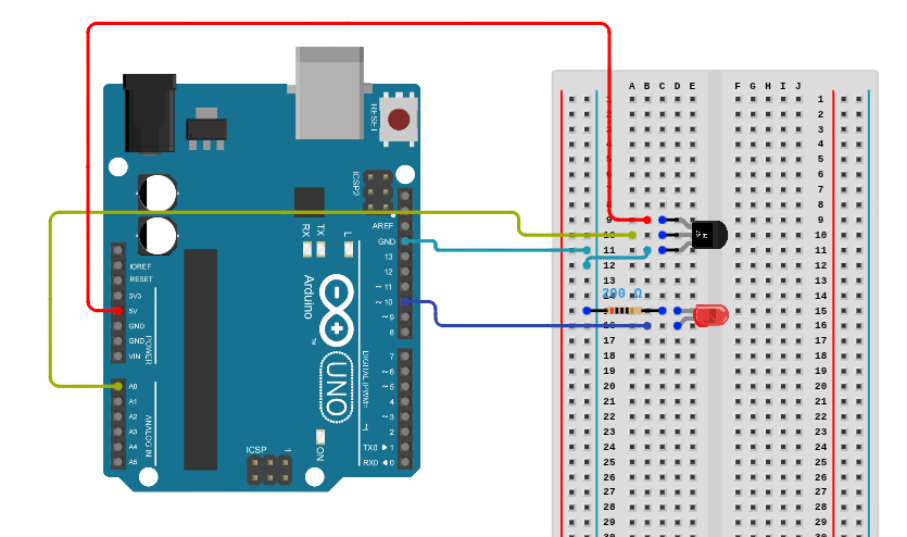
\includegraphics[width=\linewidth]{Image/2.maniptempérature}
		\caption{Schéma de l'utilisation du LM35}
		\label{fig:schema_lm35}
	\end{minipage}\hfill
	\begin{minipage}{0.48\textwidth}
		\centering
		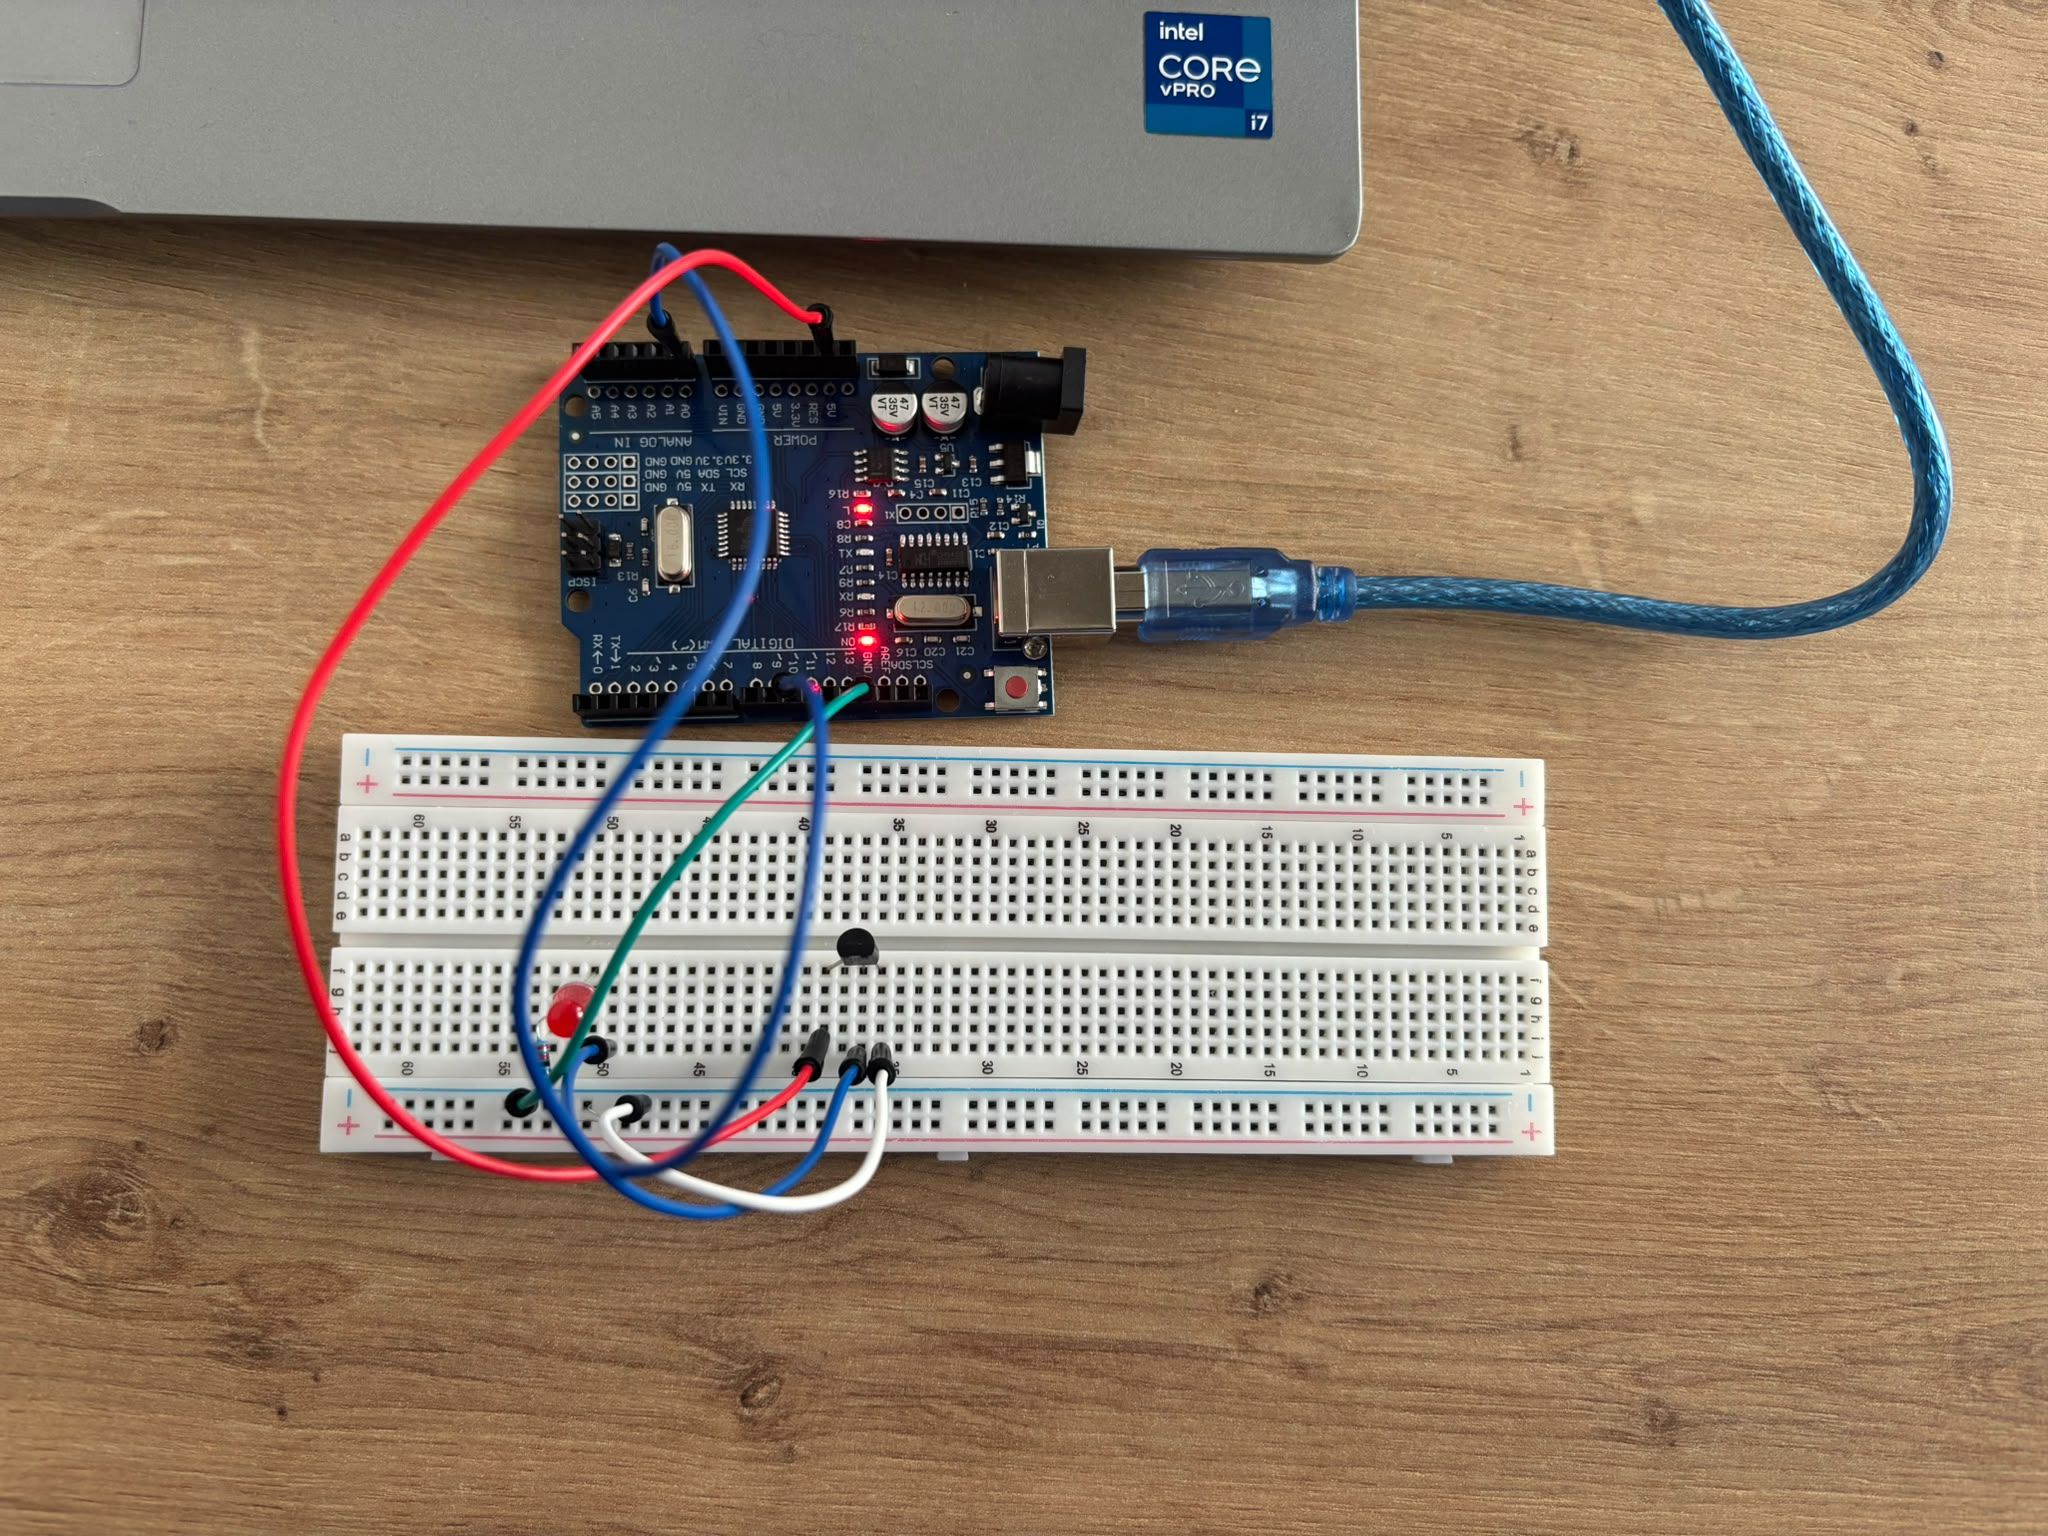
\includegraphics[width=\linewidth]{Image/2.Photomainp_température}
		\caption{Photo du montage du LM35}
		\label{fig:photo_lm35}
	\end{minipage}
\end{figure}
Pour commencer nous allons programmer la carte pour uniquement récupérer les informations du LM35.
\begin{lstlisting}				
const int lm35Pin = A0; // Broche du capteur LM35

void setup() {
	Serial.begin(9600); // Initialisation de la communication serie
}
void loop() {
	int val = analogRead(lm35Pin); // Lecture de la valeur analogique (0 a 1023)
	
	// Conversion de la valeur lue en tension (en mV), puis en temperature (C)
	
	float voltage = val * (5.0 / 1023.0);
	float temperature = voltage * 100.0; // 10 mV par C donc T = tension * 100
	
	Serial.print("Temperature : ");
	Serial.print(temperature);
	Serial.println(" C");
	
	delay(1000); // Pause d'une seconde entre chaque mesure
}
\end{lstlisting}
\textbf{Observations :} Nous utilisons le moniteur série de l'Arduino pour relever la température mesurée par le capteur. La valeur obtenue étant d'environ 22 °C, nous pouvons en déduire que le montage et la programmation ont été réalisés avec succès.
\begin{figure}[H]
	\centering
	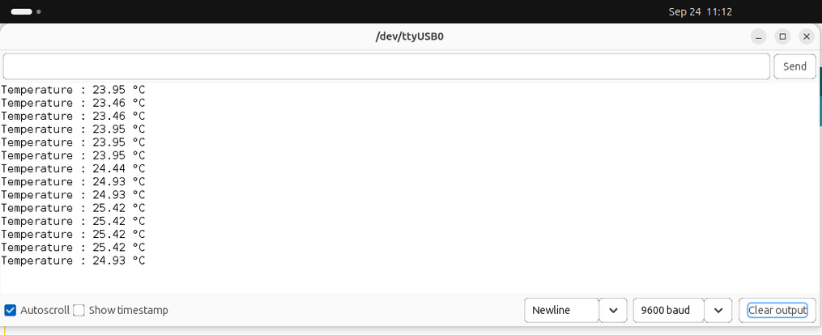
\includegraphics[width=0.7\linewidth]{Image/2.Resultat_LM35}
	\caption{Monitor série du capteur LM35}
	\label{fig:2}
\end{figure}
Nous faisons évoluer le programme pour utiliser la LED comme indicateur d'alerte. Si la température mesurée par le LM35 est supérieure à 35 °C, nous commandons l'allumage de la LED.
\begin{lstlisting}				
const int lm35Pin = A0; // Broche du capteur LM35
void setup() {
	Serial.begin(9600); // Initialisation de la communication serie
	pinMode(10, OUTPUT);
}
void loop() {
	int val = analogRead(lm35Pin); // Lecture de la valeur analogique (0 a 1023)

	// Conversion de la valeur lue en tension (en mV), puis en temperature (C)
	
	float voltage = val * (5.0 / 1023.0);
	float temperature = voltage * 100.0; // 10 mV par C donc T = tension * 100
	
	Serial.print("Temperature : ");
	Serial.print(temperature);
	Serial.println(" C");
	
	delay(1000); // Pause d'une seconde entre chaque mesure
	
	if (temperature > 29) {
		digitalWrite(10,HIGH); // on allume la LED
	}else {
		digitalWrite(10,LOW); // on eteint la LED
	}
}
\end{lstlisting}
\textbf{Observations :} Lorsque que nous plaçons notre doigts sur le LM35 alors la LED s'allume car nous dépassons le seuil de température de notre programme.
\section{Mesurer la luminosité avec une photorésistance et une carte Arduino}
Une \textbf{photorésistance} est un composant électronique dont la valeur (en ohms) varie en fonction de la lumière ambiante : \textbf{plus elle est éclairée, plus sa résistance diminue}.

\paragraph{Caractéristiques classiques}
\begin{itemize}
	\item \textbf{Dans l'obscurité :} Résistance très élevée (environ 1 M$\Omega$).
	\item \textbf{En pleine lumière :} Résistance plus faible (environ 12 k$\Omega$).
\end{itemize}

\paragraph{Applications principales}
Ce comportement permet de mesurer la luminosité ambiante pour diverses utilisations :
\begin{itemize}
	\item Détection de l'état jour/nuit.
	\item Ajustement automatique de l'éclairage.
	\item Systèmes de suivi de lumière (panneaux solaires, robotique).
\end{itemize}
\begin{figure}[H]
	\centering
	\begin{minipage}{0.48\textwidth}
		\centering
		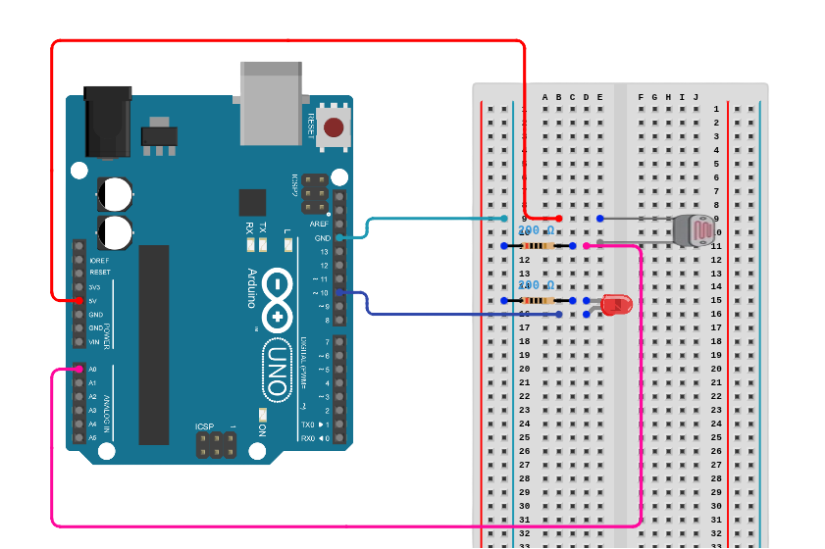
\includegraphics[width=\linewidth]{Image/2.Schéma_Manip2}
		\caption{Schéma du montage avec photorésistance}
		\label{fig:schema_photores}
	\end{minipage}\hfill
	\begin{minipage}{0.48\textwidth}
		\centering
		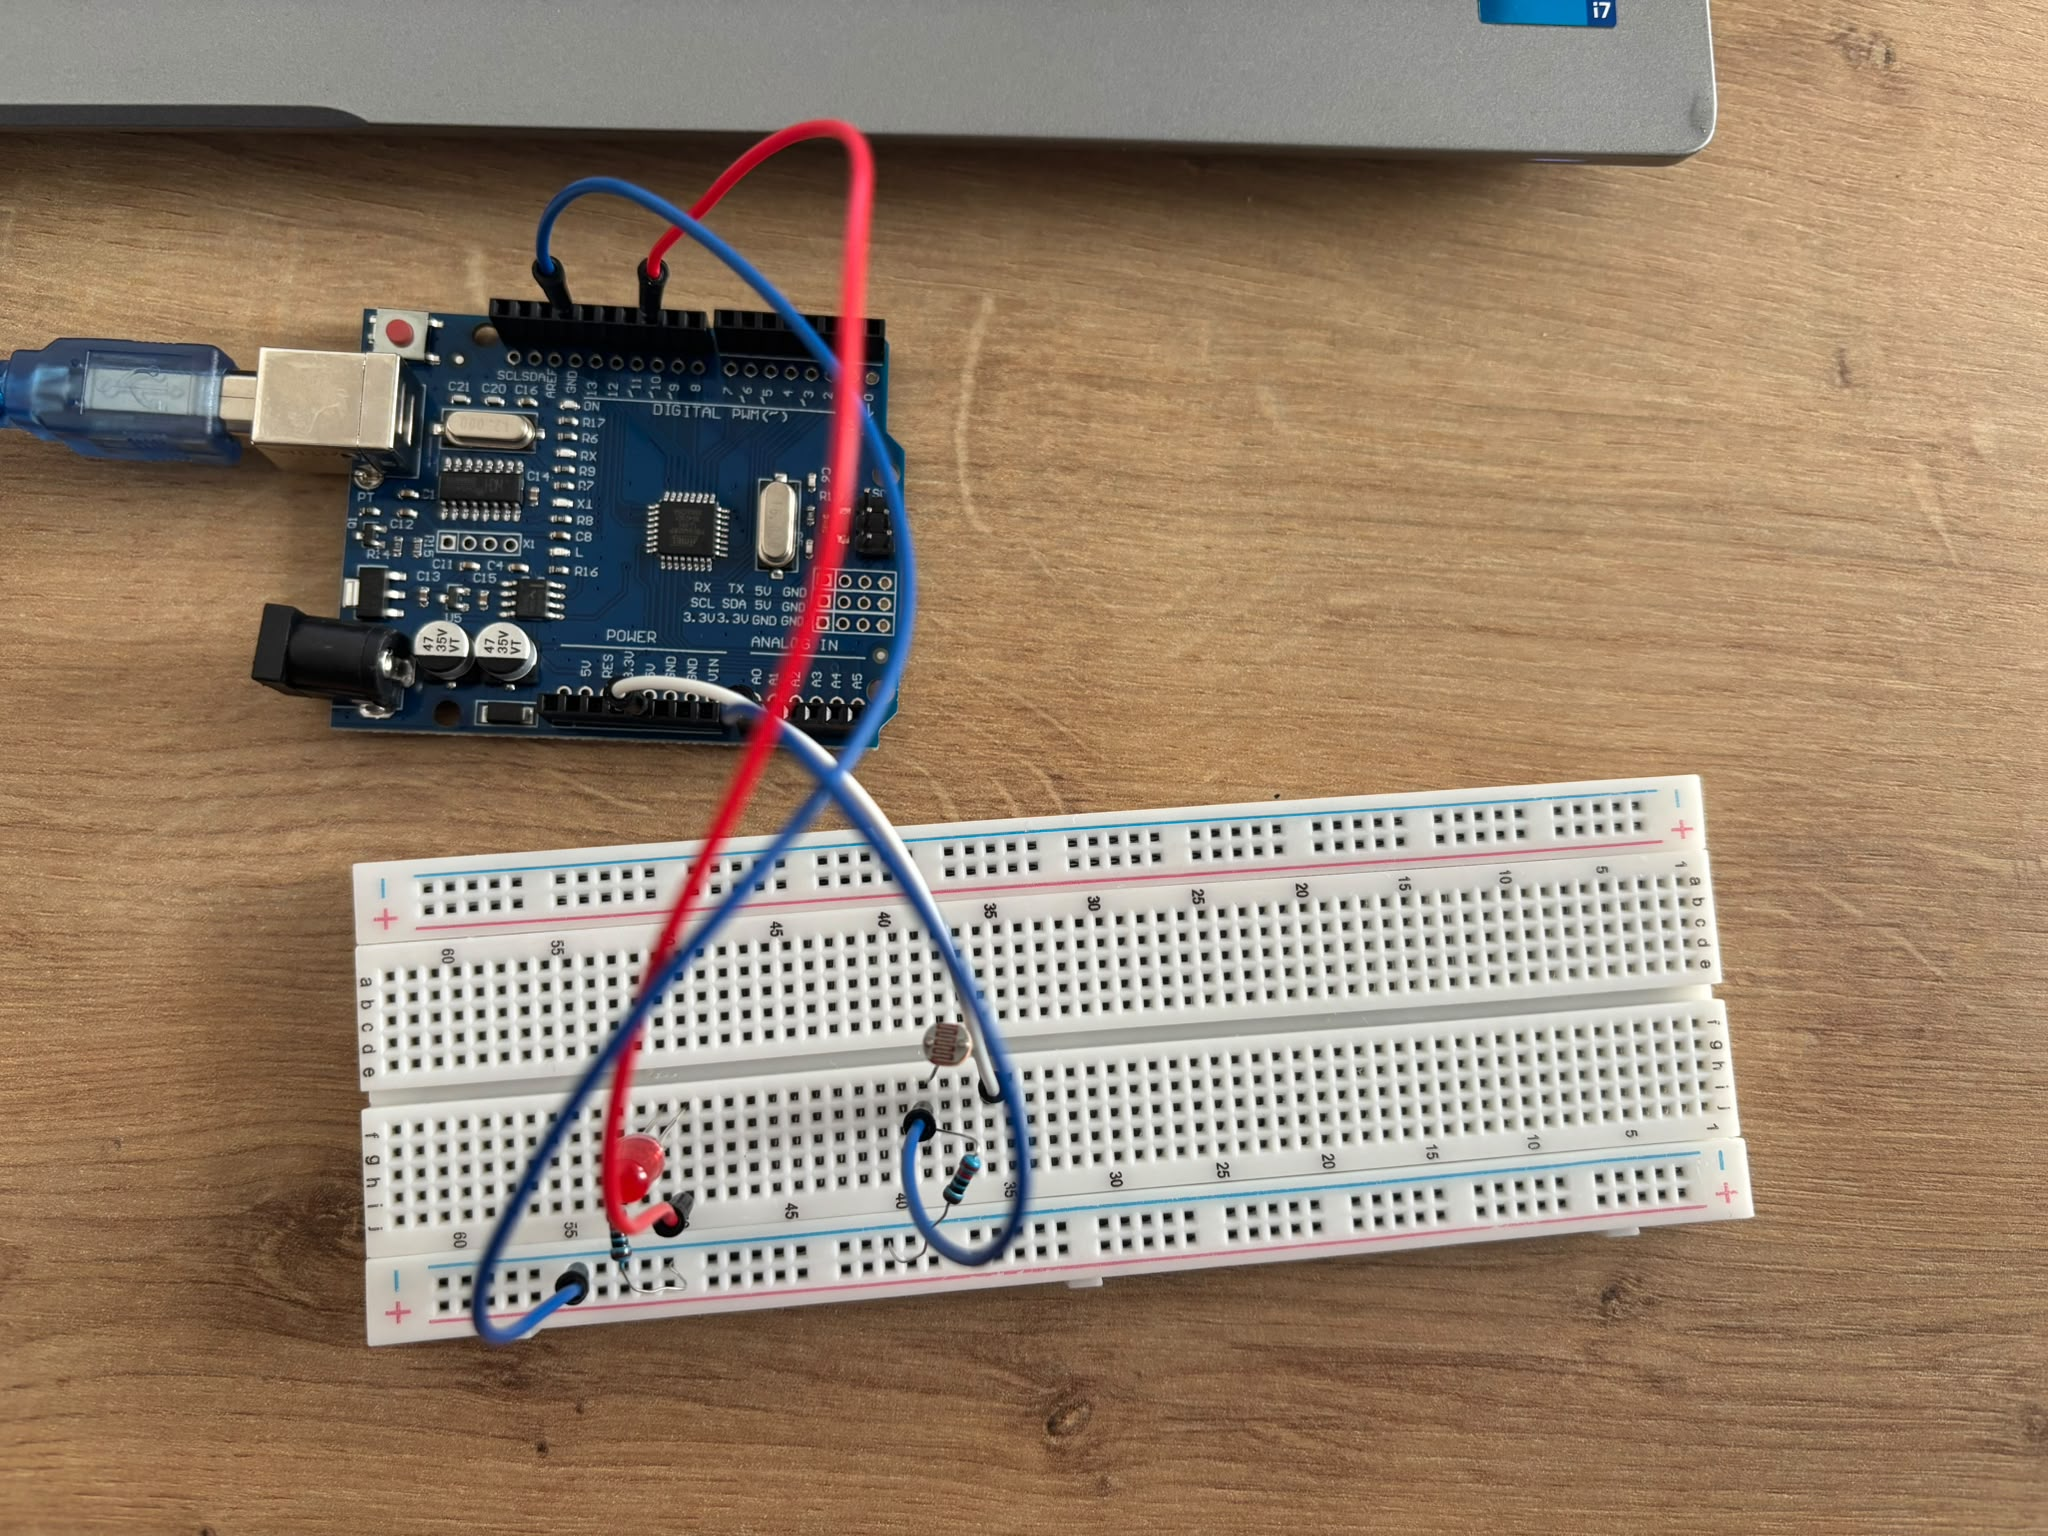
\includegraphics[width=\linewidth]{Image/2.Photo_Manip2}
		\caption{Photo montage avec la photorésistance}
		\label{fig:photo_photores}
	\end{minipage}
\end{figure}
Ensuite, nous allons faire un programme permettant de gérer l'allumage d'une LED en fonction de la luminosité reçue par la photorésistance.
\begin{lstlisting}					
	// Initialisation des constantes :
	const int analogInPin = A0; // Numero de la broche a laquelle est connectee la photoresistance
	const int analogOutPin = 10; // Numero de la broche a laquelle est connectee la LED
	
	int sensorValue = 0; // Valeur lue sur la photoresistance
	int outputValue = 0; // Valeur envoyee a la LED	
	void setup() {
		// Initialise la communication avec l'ordinateur
		Serial.begin(9600);
		// Indique que la broche analogOutPin est une sortie :
		pinMode(analogOutPin, OUTPUT);
		// Indique que la broche analogInPin est une entree :
		pinMode(analogInPin, INPUT);
	}	
	void loop() {
		// lit la valeur de la photoresistance et
		// stocke le resultat dans sensorValue :
		sensorValue = analogRead(analogInPin);
		// change sensorValue vers une intervalle de 0 a 255
		// et stocke le resultat dans outputValue :
		outputValue = map(sensorValue, 0, 1023, 0, 255);
		// envoie de cette nouvelle valeur sur la LED
		analogWrite(analogOutPin, outputValue);
		Serial.print("sensor = " );
		Serial.print(sensorValue);
		Serial.print("\t output = ");
		Serial.println(outputValue);
	}
\end{lstlisting}
\textbf{Observations :} Lorsque nous mettons notre doigt sur la photorésistance pour baiser la luminosité alors la LED s'allume.
Nous allons rajouter une autre LED qui s'allume avec un autre seuil.
\begin{figure}[H]
	\centering
	\begin{minipage}{0.48\textwidth}
		\centering
		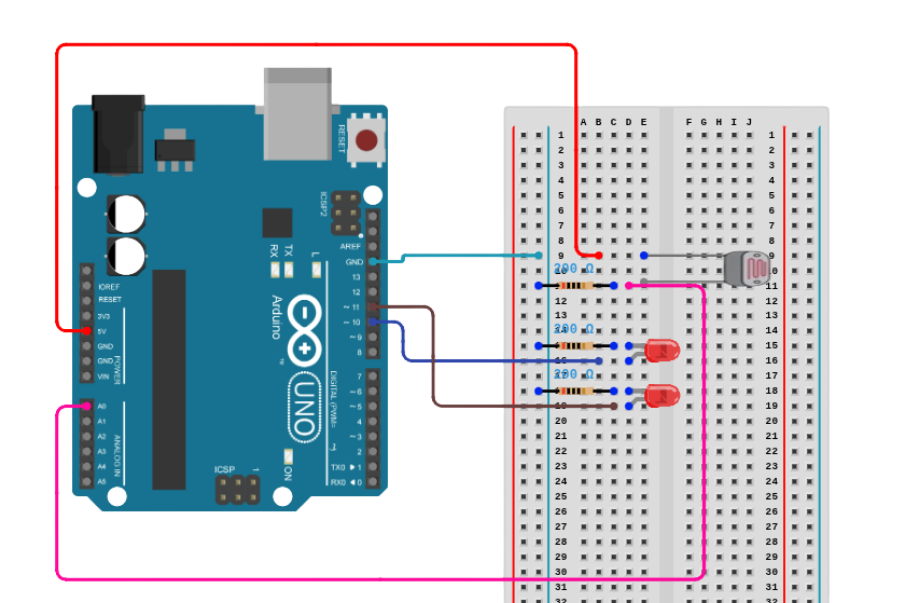
\includegraphics[width=\linewidth]{Image/2.Schéma_Manip3}
		\caption{Schéma du montage avec photorésistance et deux LED}
		\label{fig:schema_photores}
	\end{minipage}\hfill
	\begin{minipage}{0.48\textwidth}
		\centering
		\includegraphics[width=\linewidth]{Image/2.Photo_Manip3}
		\caption{Photo montage avec la photorésistance et deux LED}
		\label{fig:photo_photores}
	\end{minipage}
\end{figure}
\begin{lstlisting}					
void loop() {	
	sensorValue = analogRead(analogInPin);
	
	outputValue = map(sensorValue, 0, 1023, 0, 255);
	
	analogWrite(analogOutPin, outputValue);
	
	Serial.print("sensor = " );
	Serial.print(sensorValue);
	Serial.print("\t output = ");
	Serial.println(outputValue);	
	if(sensorValue < ((1023*1)/100) ){
		digitalWrite(11, HIGH);
	}else{
		digitalWrite(11, HIGH);
	}	
}
\end{lstlisting}
\textbf{Observations :} Les deux LED s'allume bien lorsque en fonction du seuil de luminosité atteint.
\section{Variation de la luminosité d'une LED avec un potentiomètre et une carte Arduino}
Pour terminer cette manipulation, nous intégrons un potentiomètre au lieu d'un capteur automatique. Cela nous donne la possibilité de contrôler manuellement le circuit en modifiant la valeur de sa résistance.
\begin{figure}[H]
	\centering
	\begin{minipage}{0.48\textwidth}
		\centering
		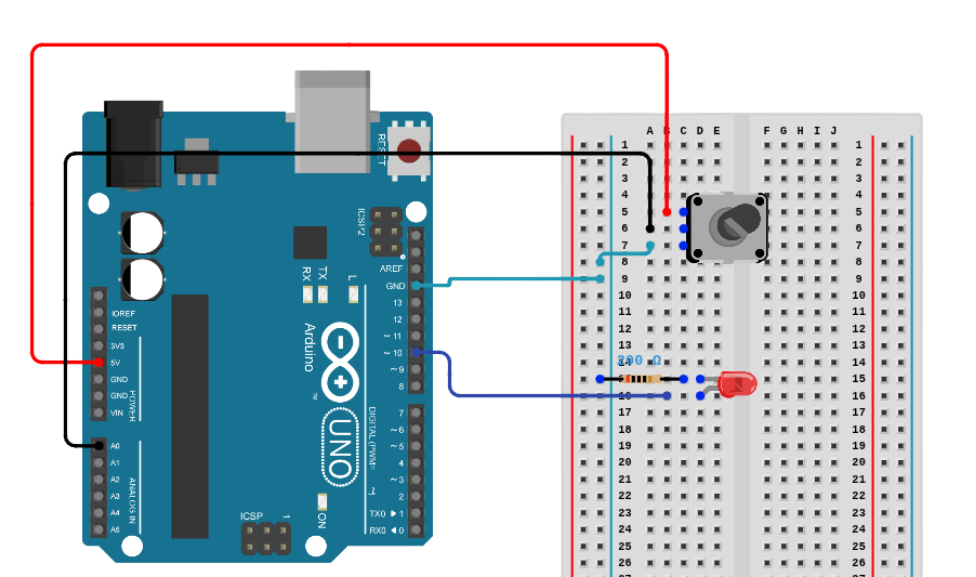
\includegraphics[width=\linewidth]{Image/2.Schéma_Manip4}
		\caption{Schéma du montage avec le potentiomètre}
		\label{fig:schema_photores}
	\end{minipage}\hfill
	\begin{minipage}{0.48\textwidth}
		\centering
		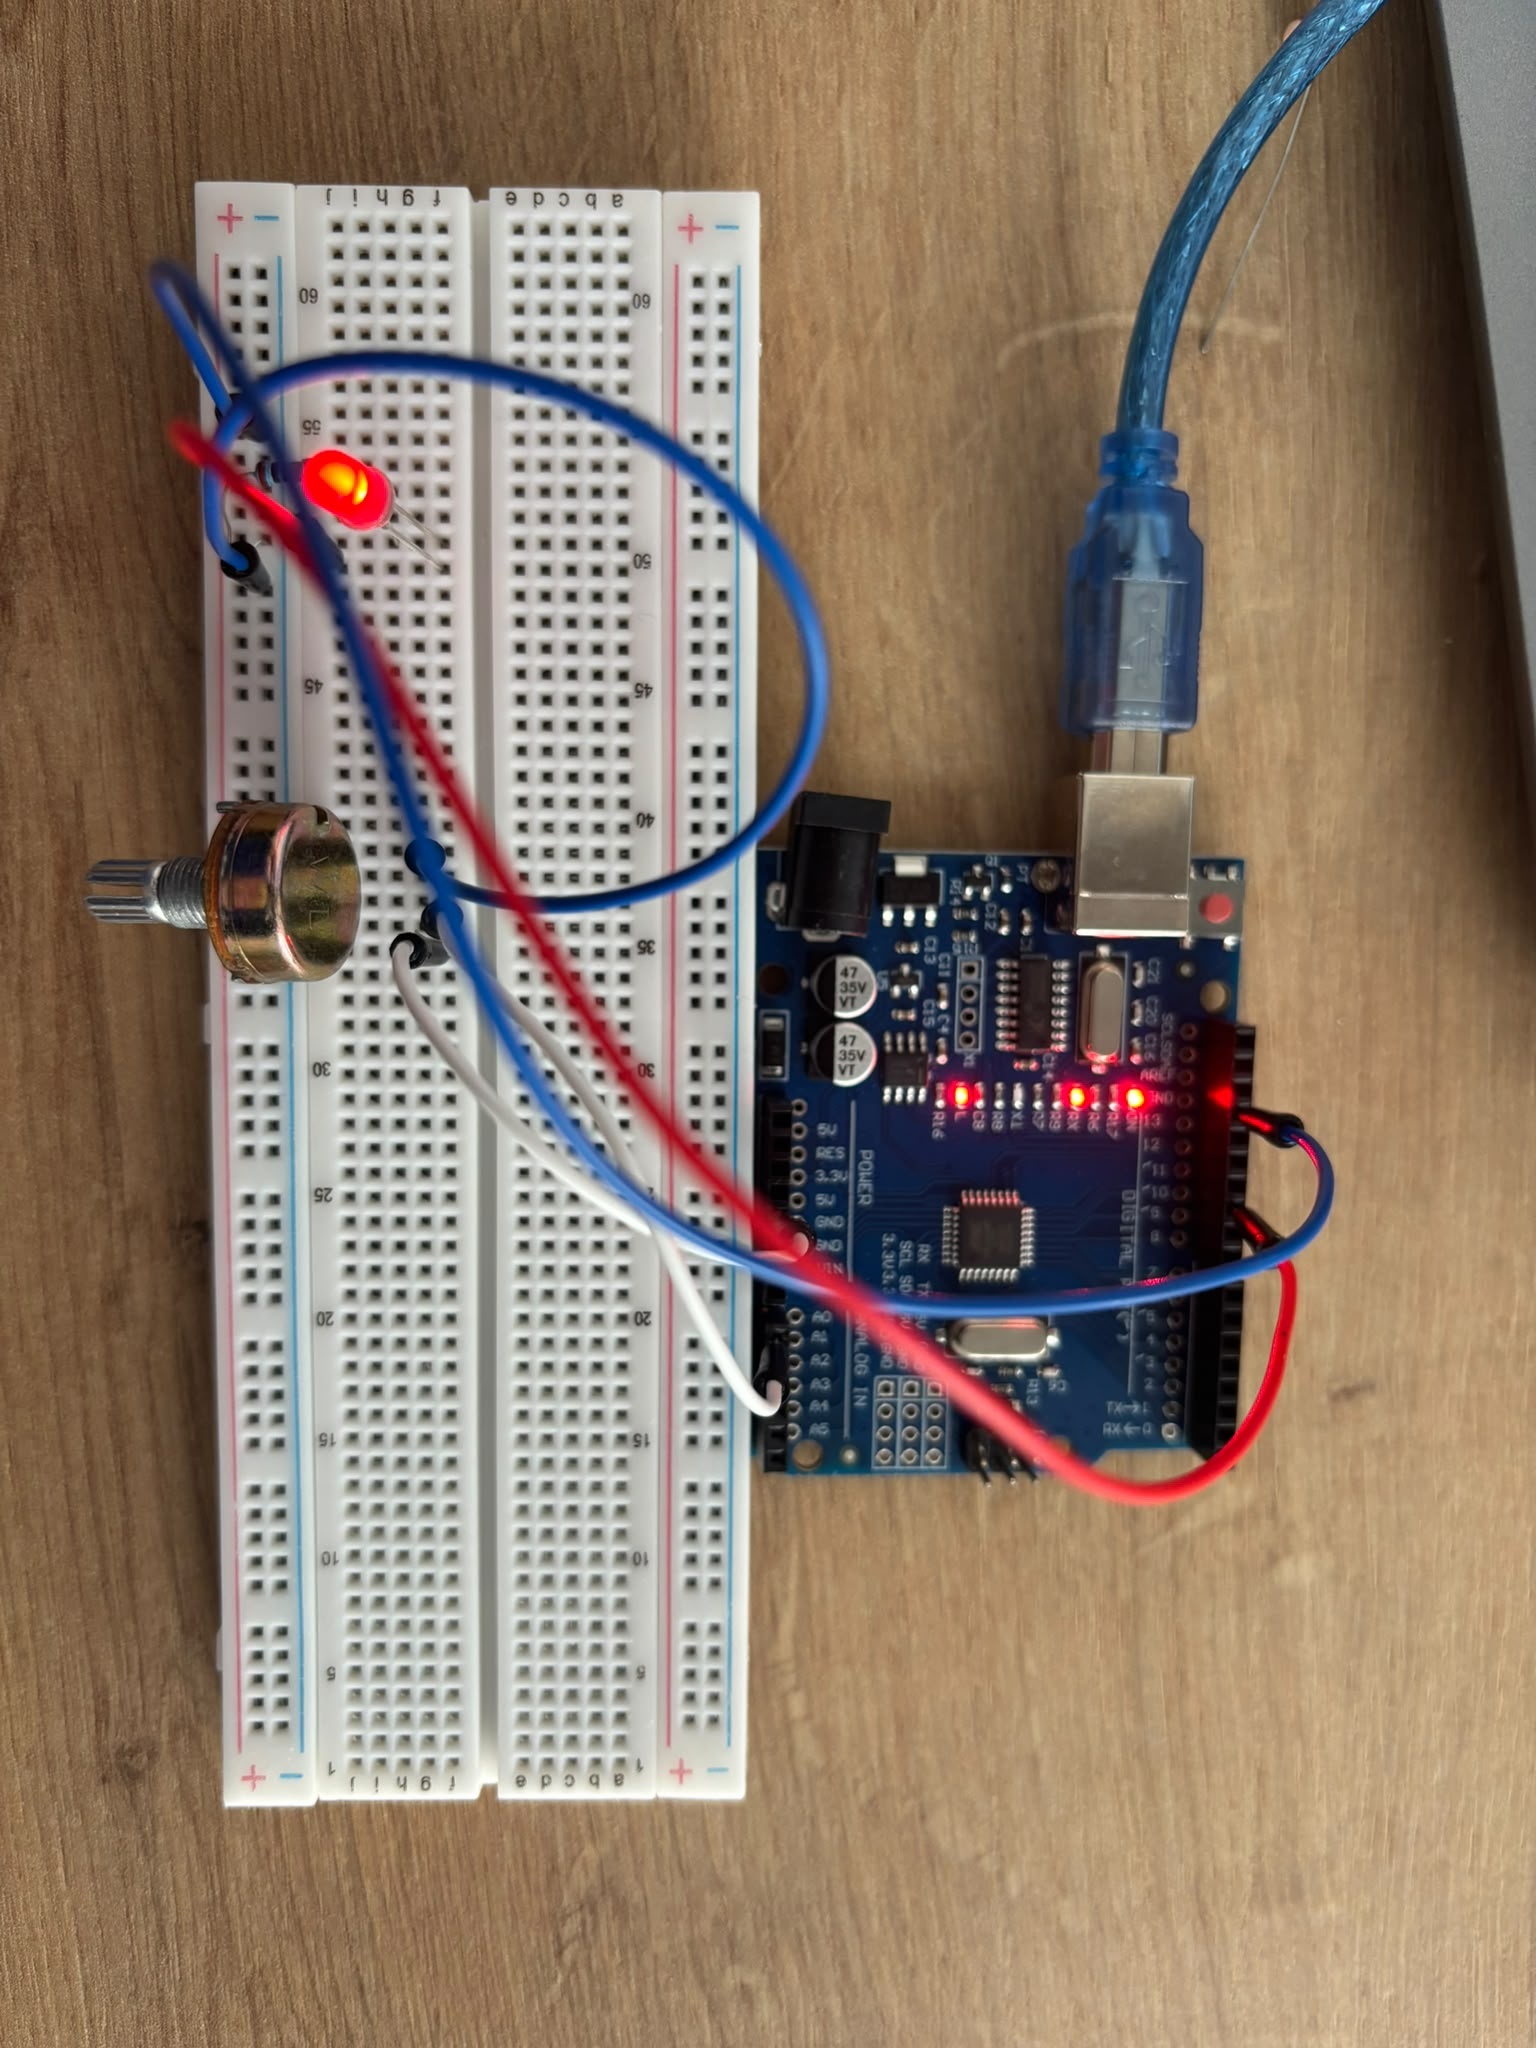
\includegraphics[width=\linewidth]{Image/2.Photo_Manip4}
		\caption{Photo montage avec le potentiomètre}
		\label{fig:photo_photores}
	\end{minipage}
\end{figure}
Nous modifions alors un peu le code de la photorésistance pour utiliser le potentiomètre.
\begin{lstlisting}					
	void loop() {
		
		sensorValue = analogRead(analogInPin);
		
		outputValue = map(sensorValue, 0, 1023, 0, 255);
		
		analogWrite(analogOutPin, outputValue);
		
		Serial.print("sensor = " );
		Serial.print(sensorValue);
		Serial.print("\t output = ");
		Serial.println(outputValue);		
	}	
\end{lstlisting} 
\textbf{Observations :} La LED s'allume bien lorsque que nous tournons le potentiomètre.\\
Nous ajoutons ensuite une autre LED qui devras s'allumer quand le potentiométre est au minimum.
\begin{figure}[H]
	\centering
	\begin{minipage}{0.48\textwidth}
		\centering
		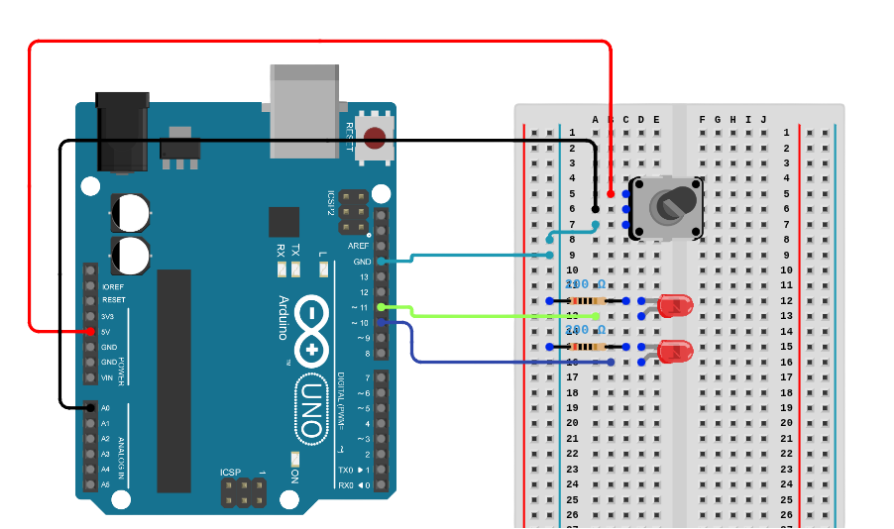
\includegraphics[width=\linewidth]{Image/2.Schéma_Manip5}
		\caption{Schéma du montage du potentiométre avec 2 LED}
		\label{fig:schema_photores}
	\end{minipage}\hfill
	\begin{minipage}{0.48\textwidth}
		\centering
		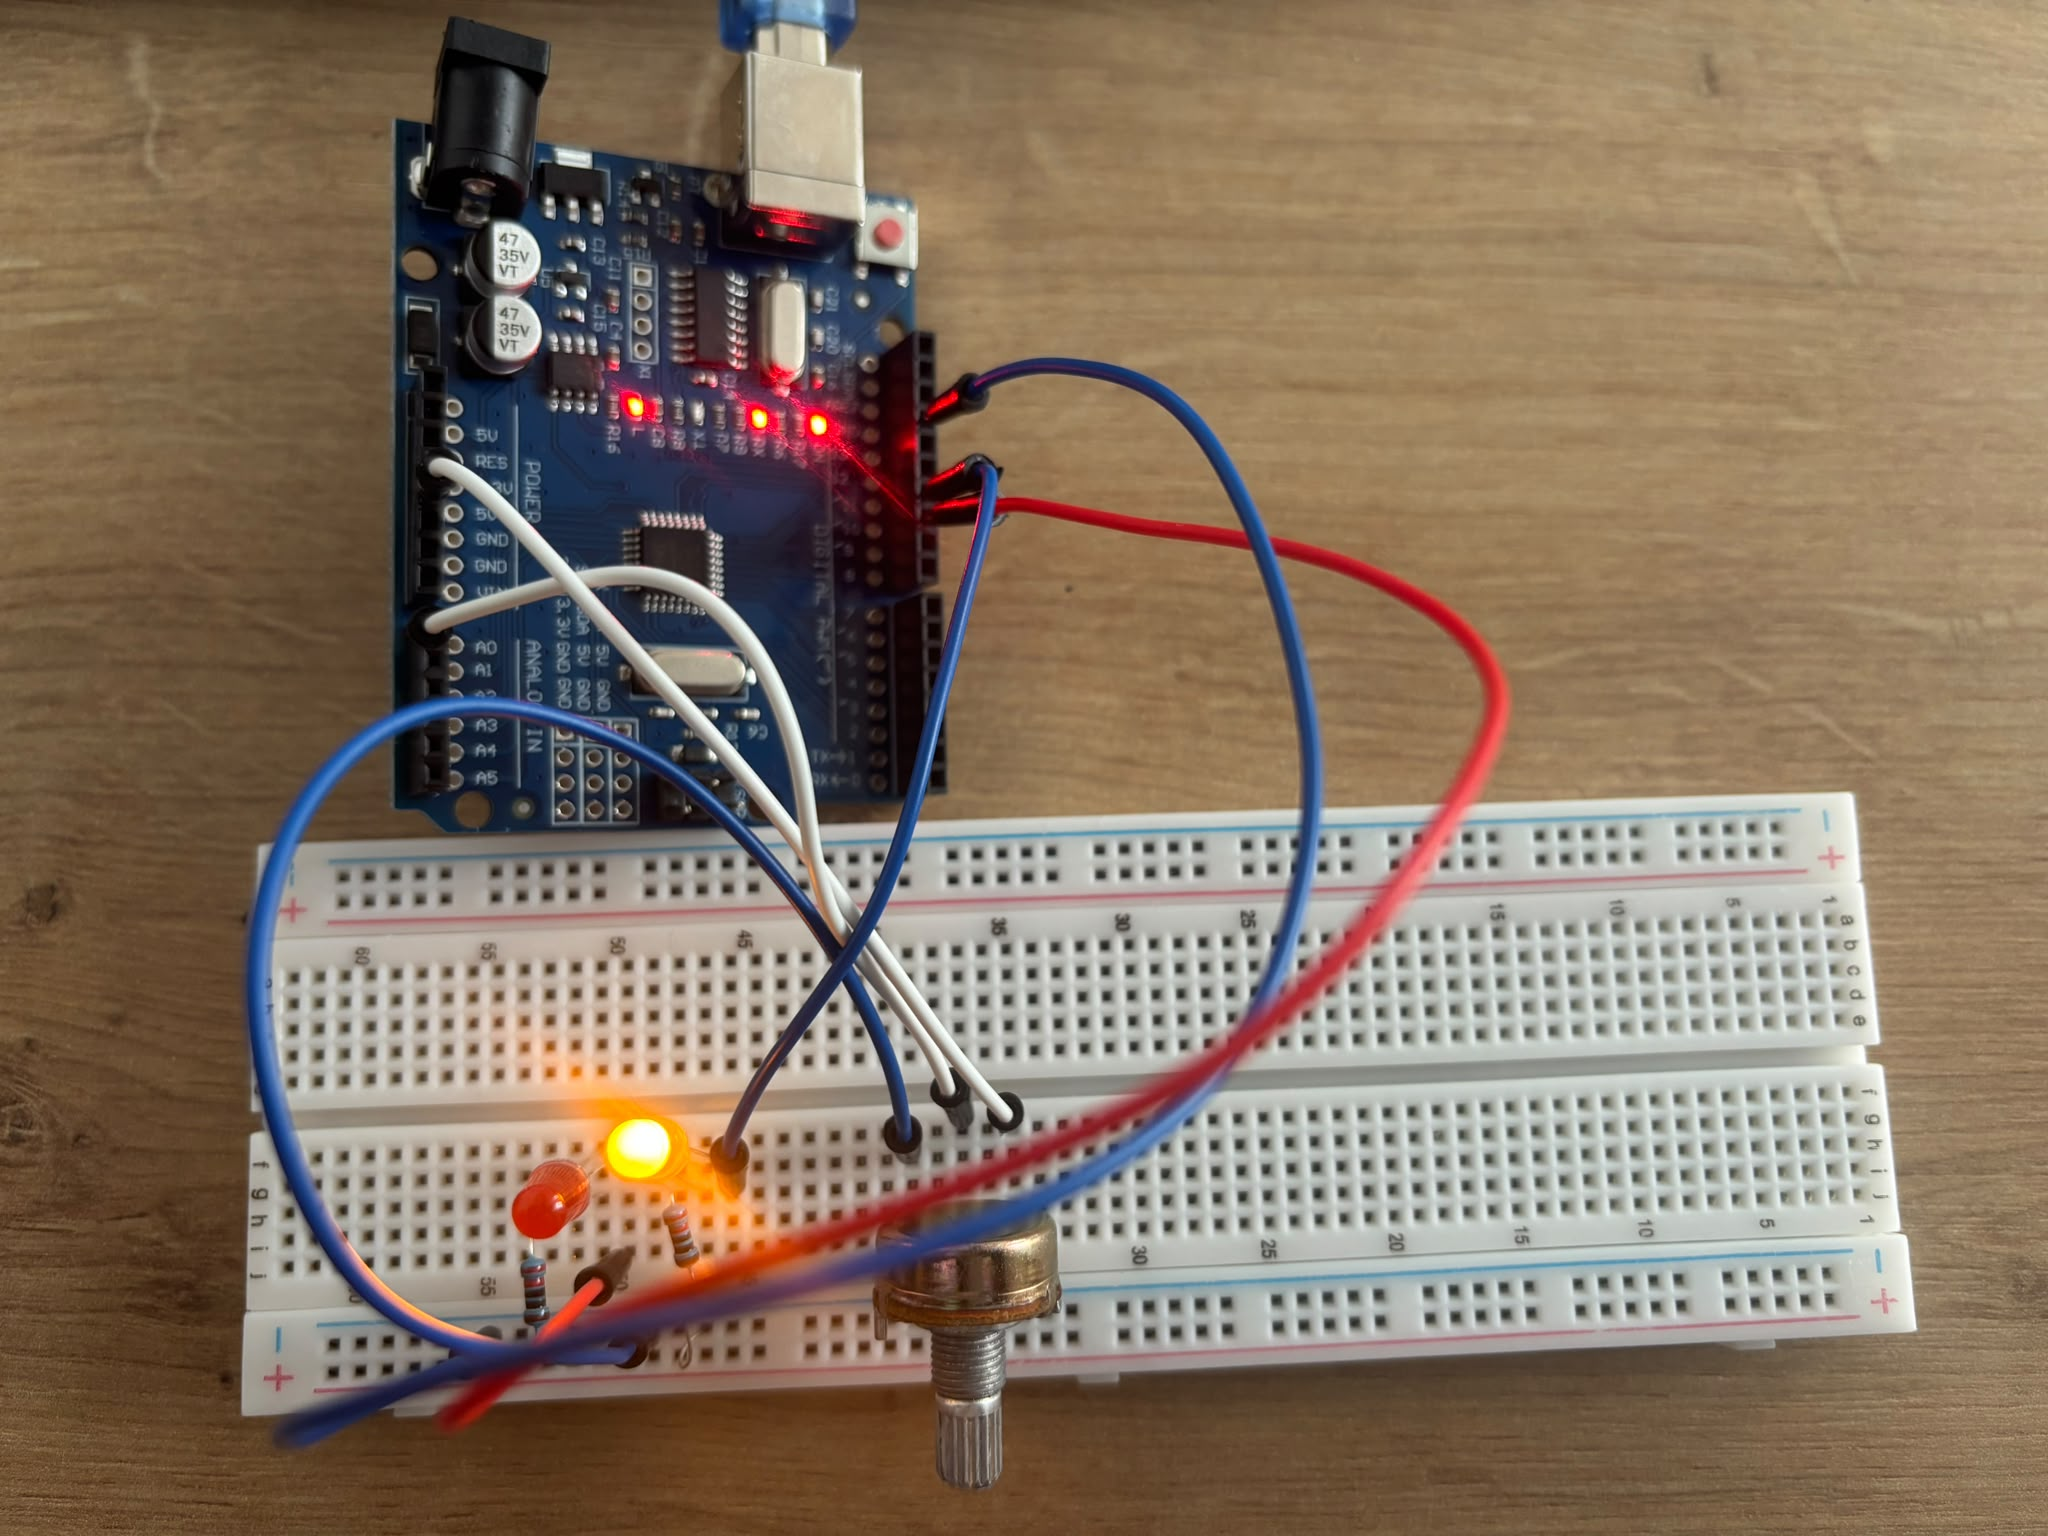
\includegraphics[width=\linewidth]{Image/2.Photo_Manip5}
		\caption{Photo montage du potentiométre avec 2 LED}
		\label{fig:photo_photores}
	\end{minipage}
\end{figure}
\begin{lstlisting}					
	void loop() {
		
		sensorValue = analogRead(analogInPin);
		
		outputValue = map(sensorValue, 0, 1023, 0, 255);
		outputValue2 = map(sensorValue, 0, 1023, 255, 0); // on inverse le 255
		
		analogWrite(analogOutPin, outputValue);
		analogWrite(11, outputValue2);
		
		Serial.print("sensor = " );
		Serial.print(sensorValue);
		Serial.print("\t output = ");
		Serial.println(outputValue);
			
	}
	
\end{lstlisting} 
\textbf{Observations :} Tourner le potentiomètre dans un sens allume une première LED, le tourner dans l'autre sens allume la seconde.\\
Pour finir avec ce TP nous devons afficher sur un écran LCD la température que nous mesurons a l'aide du LM35 utilisé dans la première partie du TP.
Pour ce faire nous utilisons un code qui a été fournie par une bibliothèque trouvé sur Google.
\begin{lstlisting}					
	#include <Wire.h>
	#include <LiquidCrystal_I2C.h>	
	const int lm35Pin = A0; // Broche du capteur LM35	
	// Initialisation du LCD I2C : Adresse 0x27, 16 colonnes, 2 lignes
	LiquidCrystal_I2C lcd(0x27, 16, 2); 
	
	void setup() {
		// Initialisation du LCD
		lcd.init();
		lcd.backlight(); // Allume le retroeclairage
		lcd.clear();
	}	
	void loop() {
		int val = analogRead(lm35Pin); // Lecture du capteur
		
		// Conversion en temperature (C)
		float voltage = val * (5.0 / 1023.0);
		float temperature = voltage * 100.0; 
		
		// Affichage sur l'ecran LCD
		lcd.setCursor(0, 0); // Ligne 1
		lcd.print("Temp: ");
		lcd.print(temperature, 1); // 1 chiffre apres la virgule
		lcd.print(" C   "); // Espaces pour eviter les bugs d'affichage
		
		delay(1000); // Pause d'une seconde avant la prochaine mesure
	}	
\end{lstlisting}  
\begin{figure}[H]
	\centering
	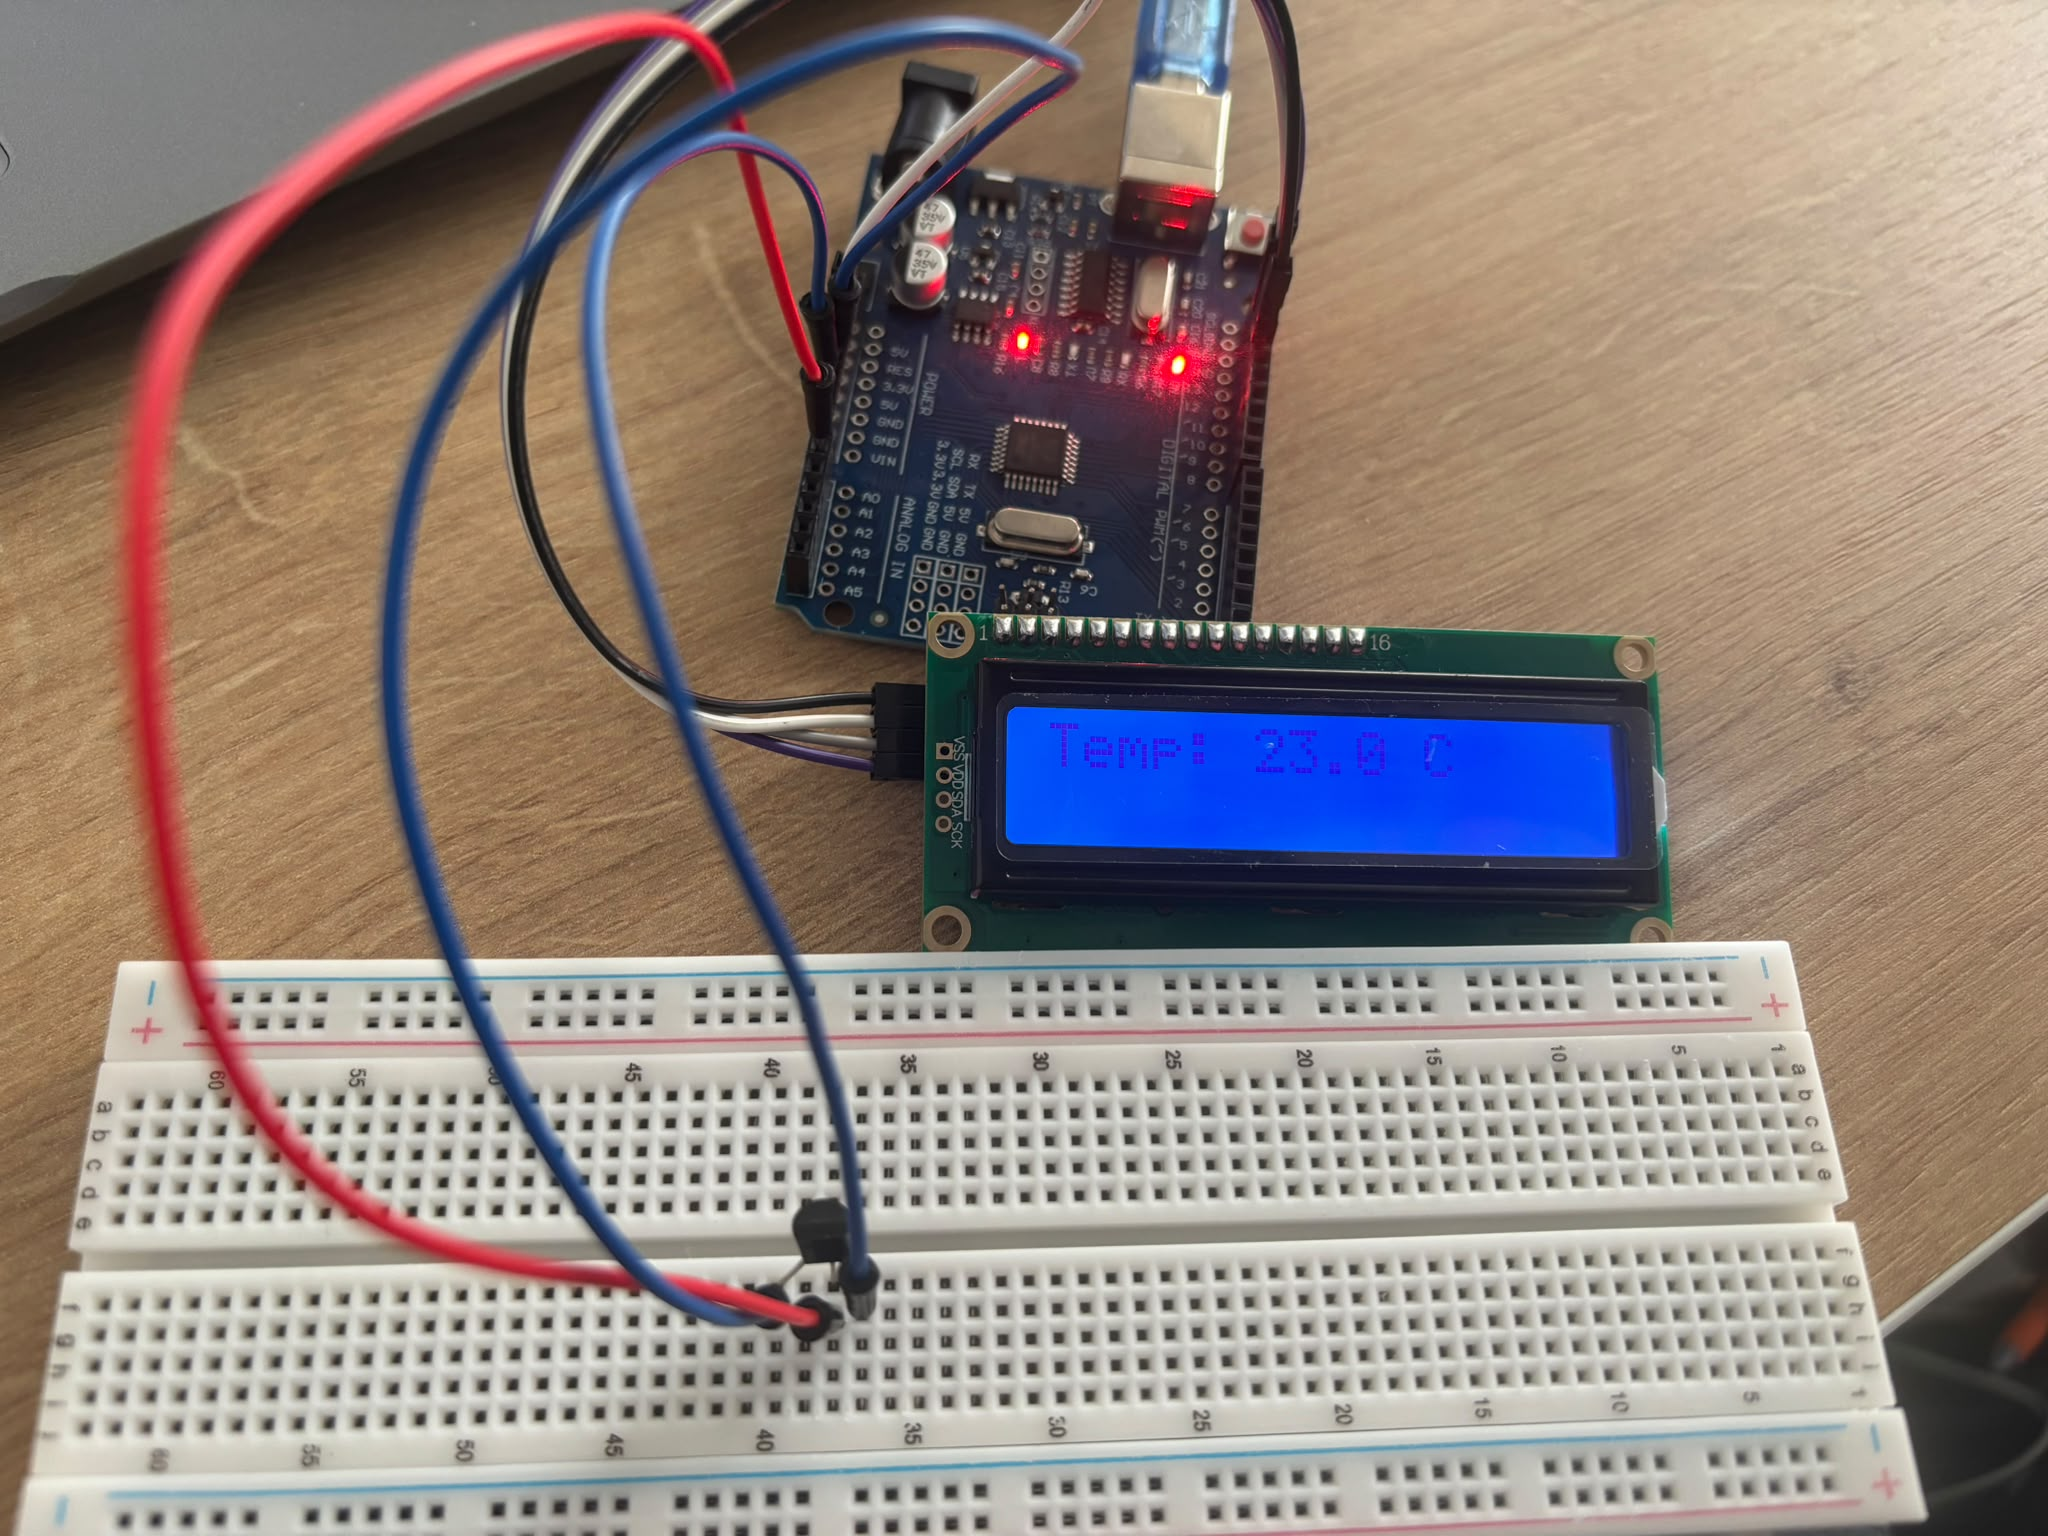
\includegraphics[width=0.7\linewidth]{Image/Photo_manip6}
	\caption{Montage de l'affichage sur l'écran LCD}
	\label{fig:photomanip6}
\end{figure}

	\end{document}